\documentclass[11pt]{article}
\usepackage{fullpage}
\usepackage{setspace}
\usepackage{amsmath}
\usepackage{fancyvrb}
\usepackage{enumerate}
\usepackage{listings}
\usepackage{pgfplots}
\usepackage{graphicx}
\usepackage{float}
\usepackage{multirow}
\usepackage[format=hang,labelsep=quad]{caption}
\usepackage{subfig}
\usepackage{array}
\usepackage{multirow}

\renewcommand\thesubfigure{\roman{subfigure}}


\begin{document}
\noindent\large{Math 5364}\\
\large{Data Mining 2}\\
\large{Homework 20}\\
\large{Mary Barker}
\doublespace
\begin{enumerate}
\item 
\begin{enumerate}
\item Perform agglomerative hierarchical clustering on the \verb|wdbc| data set, and plot the dendrogram. 

\begin{center}
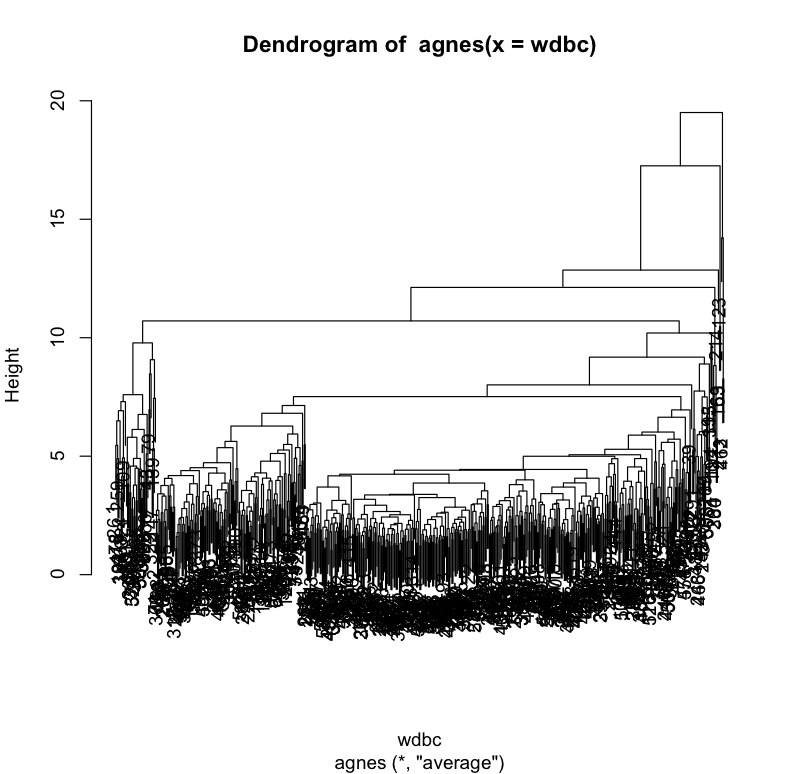
\includegraphics[scale=0.125]{dendrogram}
\end{center}

\item Cut the dendrogram to produce a clustering wtih $k = 2$ clusters.

\item Test whether the cluster labels obtained in this way are independent of diagnoses. How effective is this clustering at predicting diagnoses? 

The clustering is extremely ineffective at predicting diagnoses. 

A table of the cluster labels and diagnosis is shown below. Regardless of diagnosis, the majority of rows of data were clustered into one cluster. 

\begin{center}
\begin{tabular}{| c | c | c |}
\hline
      & cluster 1 & cluster   2 \\ \hline
   B & 357 &   0 \\ \hline
   M & 209 &   3 \\ \hline
\end{tabular}
\end{center}

\end{enumerate}

\end{enumerate}

\pagebreak
\begin{center}
\textbf{Source Code}
\end{center}
\lstinputlisting[language=R, basicstyle=\ttfamily\scriptsize]{hw20.R}

\end{document}
